%%%%%%%%%%%%%%%%%%%%%%%%%%%%%%%%%%%%%%%%%%%%%%%%%%%%%%%%%%%%%%%%%%% 
%                                                                 %
%                            CHAPTER                              %
%                                                                 %
%%%%%%%%%%%%%%%%%%%%%%%%%%%%%%%%%%%%%%%%%%%%%%%%%%%%%%%%%%%%%%%%%%% 

\chapter{Platforms for accelerating Smith-Waterman}
\label{ch:Platforms}

As we saw in the analysis of the Smith-Waterman algorithm in \ref{expl:SWanalyse}, we can see that the value of each cell in the matrix is only dependent on the left-upmost 3 cells. Therefore, It leads us to believe that this algorithm can be accelerated on other hardware solutions which are better equipped for parrallellism than a normal CPU.

\section{Overview of possible hardware}



\begin{figure}[H]
	%src=https://docs.microsoft.com/en-us/azure/machine-learning/service/media/concept-accelerate-with-fpgas/azure-machine-learning-fpga-comparison.png
	\centering
	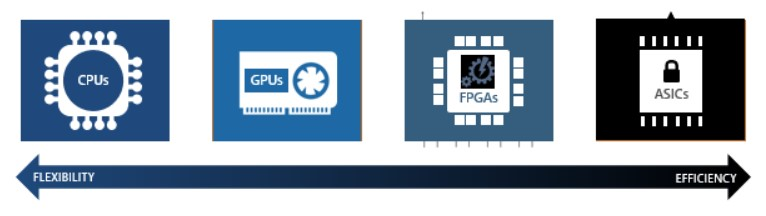
\includegraphics[width=0.75\textwidth]{elBackground/effVSflex.jpg}
	\caption{An overview of the different semiconductor technologies}
	\label{fig:effVSflex}
\end{figure}

\subsection{CPU}

//limitations CPU

Since the original implementations on CPU, it became clear that a CPU was not the most suitable platform for this algorithm, since it consists of a lot of operations which can be done in parallel. However, since the rise SIMD, CPU's have made a comeback. \emph{SIMD} stands for \emph{Single Instruction Multiple Data} and makes it possible to manipulate more than 1 attribute of data with one single instruction, although be it the same instruction on all the data. CLC bio, a Danish company specialised in bioinformatics, has been able to achieve impressive speedups with a software implementation using SIMD, closing in on 200x.
%src:https://web.archive.org/web/20070811101052/http://www.clccell.com/download.html

Nowadays, MIT has published \emph{diagonalsw}, which an implementation of S-W using the SIMD instruction set, and is licensed under the open-source MIT license.

\subsection{GPU}

//hoe werkt GPU

Since the Smith-Waterman algorithm is basically a big matrix manipulation, it lead researchers to believe that it could be accelerated on a GPU. In 1997, an implementation of S-W on a GPU was published %src:  https://archive.org/details/computationalsci0000iccs_y9o8/page/230
which achieved a speedup of 2x over all previous software implementations.

At the time of writing, 11 different implementations for Smith Waterman have been reported, 3 of which reporting a speedup over 30 times.

\subsection{FPGA}

//info over wat FPGA is.

In a paper form 2007, an implementation with an FPGA (virtex-4) achievede a speedup up to 100x over a 2.2GHz Opteron processor. %src https://ft.ornl.gov/~olaf/pubs/RSSIOlafDave.pdf
A few companies also have made some implementations of FPGA in the past, e.g. Cray Inc., TimeLogics, ...
%cray: https://www.cray.com/
%timelogics: http://www.timelogic.com/

A master's thesis from 2011 by Vermij E. has a detailed analysis of an FPGA based Smith-Waterman implementation. In other papers, it was found that the performance per Watt level for an FPGA implementation is better than a GPU or CPU by a factor of 12-21 times.

\section{Hardware selection}

\subsection{Recent advances in High Level Synthesis}

\subsection{Platform communication}
niet belangrijk
via SD
ev. Ethernet: FTP

reading from sd card so not a lot of information exchange needed
if necessary => FTP if needed

